%!TEX root = lec08_nosql.tex


%
%--------------------------------------------------------------------------------------------------------------
%

\begin{frame}{Data Partitioning}

\begin{columns}[onlytextwidth]
\begin{column}{0.5\textwidth}
Partitioning a table $R(a, b, c, d)$ within a cluster, can help \emph{balance} the storage and query/update workload across nodes.
\end{column}
\begin{column}{0.5\textwidth}
\begin{center}
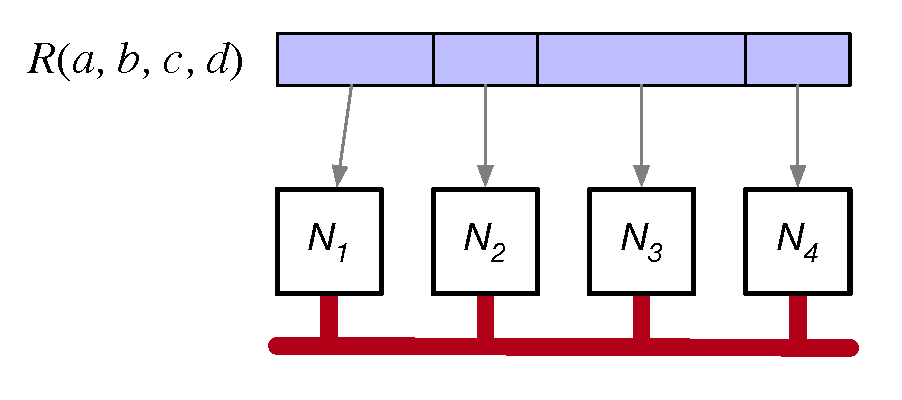
\includegraphics[width=\textwidth]{figures/table_partition_shared_nothing.eps}
\end{center}
\end{column}
\end{columns}

\vskip2em

\begin{itemize}[-,topsep=-10pt]
\item Based on \alert{ranges} of one or more partition attributes.\\
 Example, partition on $R(a)$: 
\(
\texttt{node}(t) = \left\{\begin{array}{cc}
                N_1 & t.a < k_1\\
                N_2 & k_1 \leq t.a < k_2\\
                ... & 
        \end{array}\right.
\)

\item Based on \alert{hashing} of one or more partition attributes.\\
 \(
 \texttt{node}(t) =  h(t.a) \bmod 4
 \)

\item In a round-robin fashion (i.e., tuples go to nodes based on the order they are inserted).
\end{itemize}
\end{frame}

%
%--------------------------------------------------------------------------------------------------------------
%

\begin{frame}{Cost of Finding a Tuple}

\begin{columns}[onlytextwidth]
\begin{column}{0.7\textwidth}
Recall that \blue{the costs of querying, deleting and updating a tuple all depended on the cost of finding a tuple} in t{e first place.}
\end{column}
\begin{column}{0.4\textwidth}
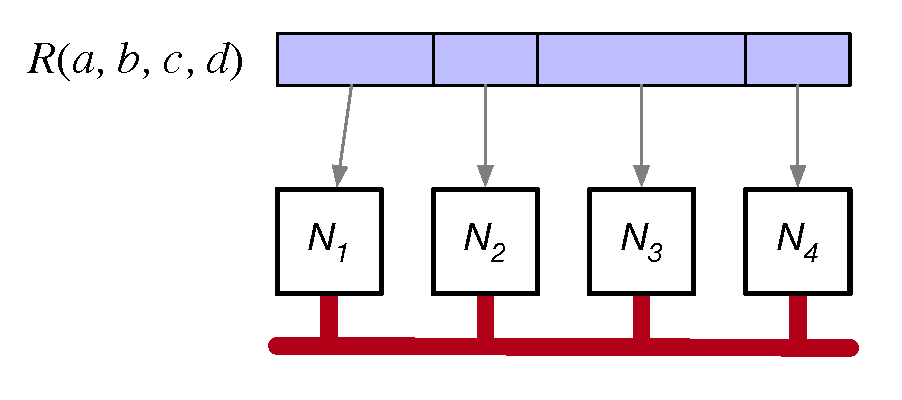
\includegraphics[width=0.75\textwidth]{figures/table_partition_shared_nothing.eps}
\end{column}
\end{columns}

\vskip1em

\alert{Cost of search based on $R(a) = v_1$}.
\begin{enumerate}[(1)]
\item Finding the node with the tuple:
\begin{itemize}[-,topsep=-10pt,noitemsep]
\item If $a$ is the partition attribute (range partition or hashing), we can quickly find the single node where the tuple is.
\item With round-robin partition \textbf{or} if $a$ is not the partition attribute, we need to search for the tuple in every node.
\end{itemize}
\item Performing the search in each node: $O(|R|)$ or $O(\log_k |R|)$ depending on whether there is an index on $a$.
\end{enumerate}

\end{frame}


%
%--------------------------------------------------------------------------------------------------------------
%

\begin{frame}{Data Distribution}

How many tuples will there be in each partition of $R$ into $R_1\cup R_2 \cdots\cup R_n$

\begin{itemize}[-,topsep=-0.5em]
\item With \textbf{round-robin}: \(T(R_i) = \dfrac{1}{N}\).
\item With \textbf{range partitioning} and with \textbf{hash partitioning}, it depends on how the distribution of the values of the partition attribute(s).
\begin{itemize}[-]
\item If the values of $R(a)$ are \blue{uniformly distributed} and $V(R,a) > N$, then \(T(R_i) = \dfrac{1}{N}\).
\item But what if they are not?
\end{itemize}
\end{itemize}
\end{frame}

%
%--------------------------------------------------------------------------------------------------------------
%

\begin{frame}

If the values of $R(a)$ are \alert{not uniformly distributed} then hashing and range partitioning will assign (possibly a lot) more tuples to a few nodes, causing the load in the cluster to be \textbf{unbalanced}.

\textbf{Ex:} suppose we partition \lstinline!Movie(title, year, imdb, director)! by year (left) or imdb score (right):

\vskip1em

\begin{columns}[onlytextwidth]
\begin{column}{0.5\textwidth}
\includegraphics[width=\textwidth]{figures/histogram_year_skew.png}
\end{column}
\begin{column}{0.5\textwidth}
\includegraphics[width=\textwidth]{figures/histogram_imdb_skew.png}
\end{column}
\end{columns}

\begin{block}{\alert{Load imbalance is a problem}}
Nodes with more data perform \textbf{a lot more} work over time.
\end{block}
\end{frame}

%
%--------------------------------------------------------------------------------------------------------------
%

\begin{frame}{Virtual nodes}

One way to combat load imbalance is to add a level of indirection by using more \emph{virtual nodes} than real nodes:
\begin{itemize}[-,noitemsep,topsep=-9pt]
\item Use any partition scheme to assign tuples to virtual nodes.
\item Assign virtual nodes to real nodes in a round-robin fashion\footnote{The other two techniques would work as well.}.
\end{itemize}

\vskip2.5em

\begin{columns}[onlytextwidth]
\begin{column}{0.5\textwidth}
In effect, using \emph{virtual} nodes is the same as increasing the granularity of the data partitioning strategy. 
\vskip0.5em

Randomizing the assignment of virtual nodes to physical nodes 
\end{column}
\begin{column}{0.5\textwidth}
\includegraphics[width=\textwidth]{figures/histogram_year_skew_fine.png}
\end{column}
\end{columns}
\vspace*{-5pt}
\noindent balances out the workload of the physical nodes.

~
\end{frame}


%
%--------------------------------------------------------------------------------------------------------------
%

\begin{frame}
\vskip2em

\begin{columns}[onlytextwidth]
\begin{column}{0.5\textwidth}
Each virtual node corresponds to a narrower slice of the data.

\vskip1em

Each physical node is assigned multiple slices, in a way that the total load in each physical node is as egalitarian as possible.

\vskip1em

Ideally, each physical node should have

\[T(R)/N \text{ tuples.}\]
\end{column}

\qquad \begin{column}{0.5\textwidth}
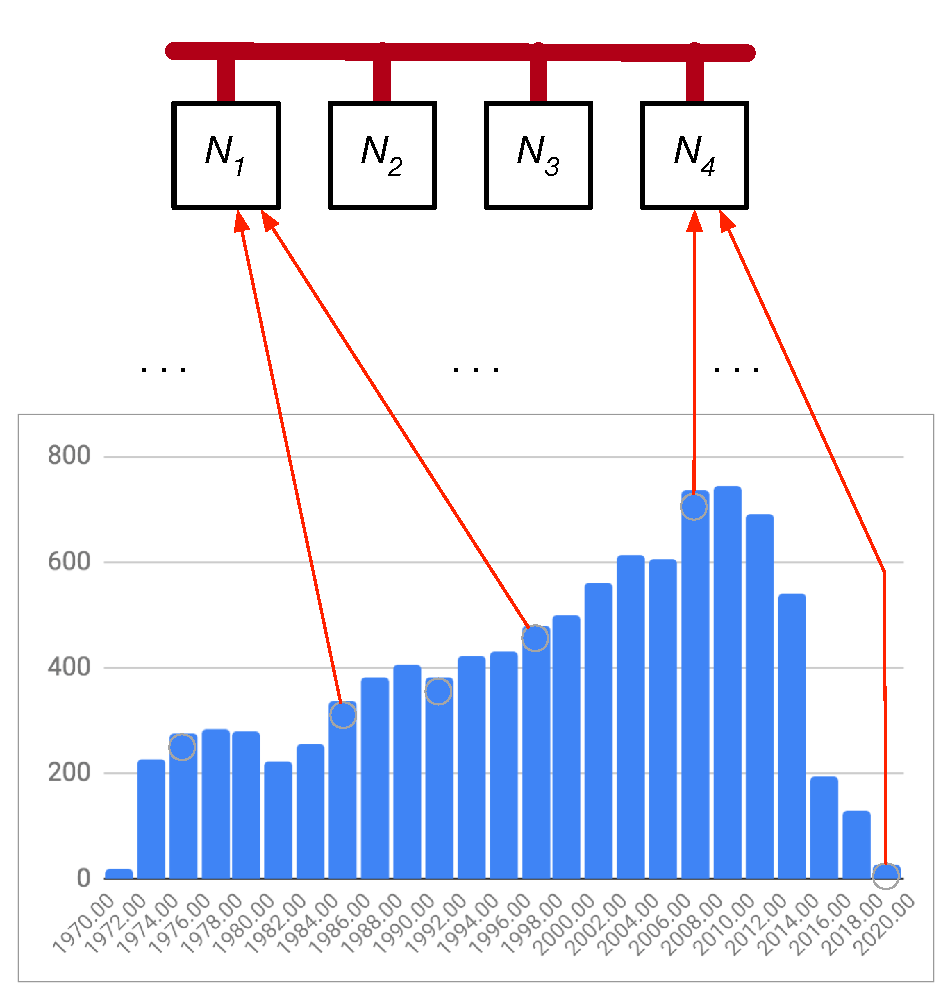
\includegraphics[width=\textwidth]{figures/virtual_node_rebalance.eps}
\end{column}
\end{columns}
\end{frame}

%
%--------------------------------------------------------------------------------------------------------------
%

\begin{frame}{Elasticity}

The use of virtual nodes to partition the data is consistent with the ``elastic nature'' of cloud computing:
\begin{itemize}[-]
\item When the cluster grows (i.e., new physical nodes are added), existing virtual nodes can be re-assigned and migrated.
\item Also, each ``slice'' of the data can be further divided into even narrower slices to help re-balance the load among physical nodes.
\end{itemize}
\end{frame}

%
%--------------------------------------------------------------------------------------------------------------
%

\begin{frame}{Replication, Redundancy and Availability}

Nodes in a cluster are \alert{expected to fail} often and without warning. 

A good way to \textbf{avoid data loss} is to keep multiple copies of the data, so that even the failure of a few nodes does not mean the entire table is lost.

\begin{center}
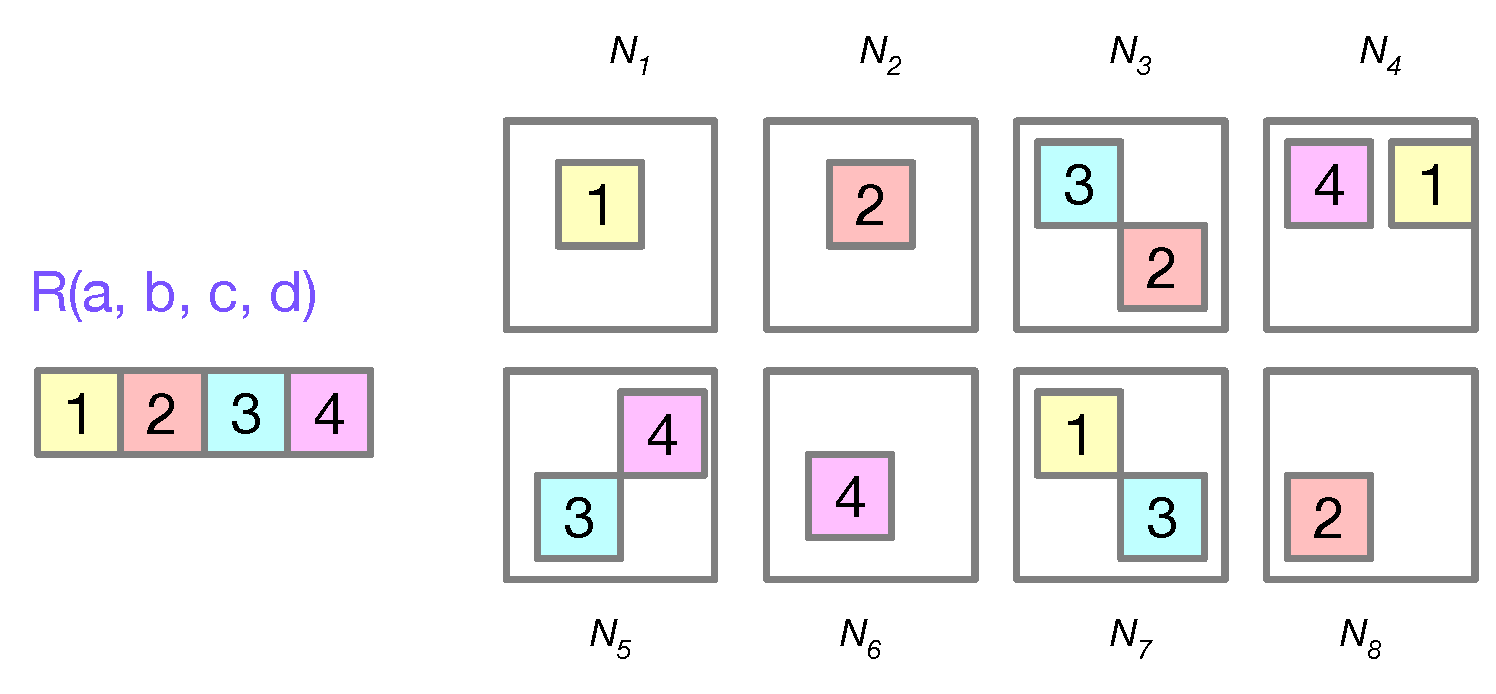
\includegraphics[width=0.75\textwidth]{figures/partitioned_table_redundancy.eps}
\end{center}

This also helps with query answering: always send request to read data to the nodes with least load.

\end{frame}


%
%--------------------------------------------------------------------------------------------------------------
%

\begin{frame}{Prototypical ``Table Store''}


The table is partitioned into \alert{tablets}, distributed and replicated across tablet servers. A \alert{directory} process, running in the \textbf{primary node} of the cluster, keeps a mapping between tablets to nodes. 

To increase availability and redundancy, directory process is replicated in multiple nodes, each running a \alert{data router} process.

\vskip1.5em

\begin{center}
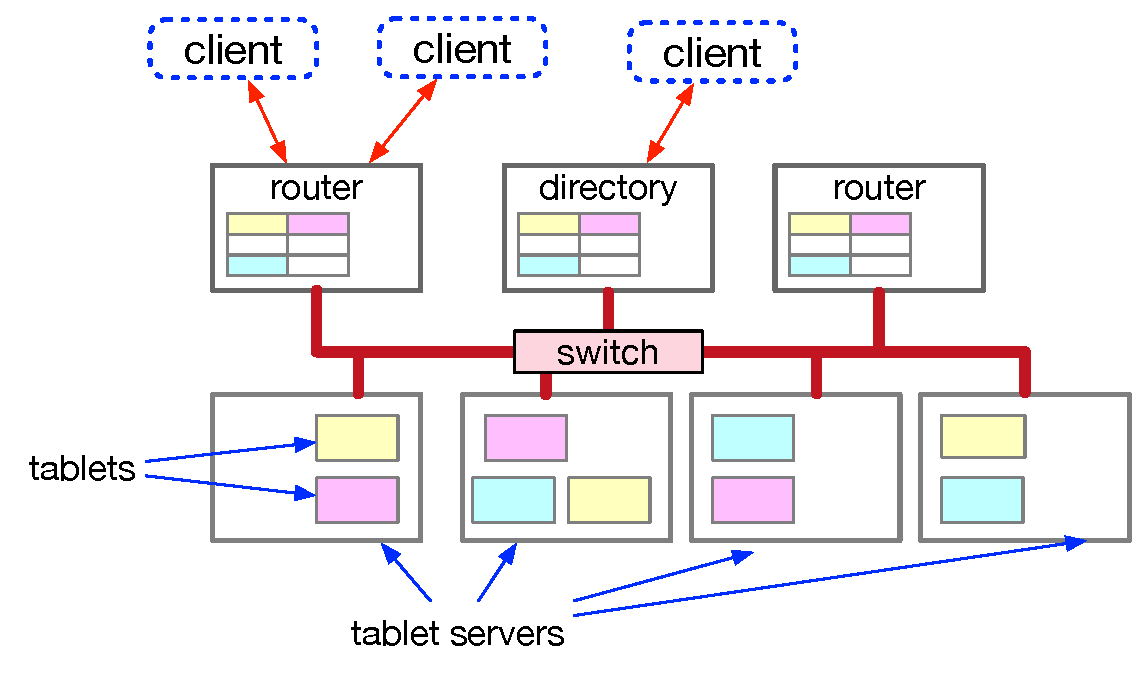
\includegraphics[width=0.75\textwidth]{figures/table_store_architecture.eps}
\end{center}

\end{frame}

%
%--------------------------------------------------------------------------------------------------------------
%

\begin{frame}

\begin{center}
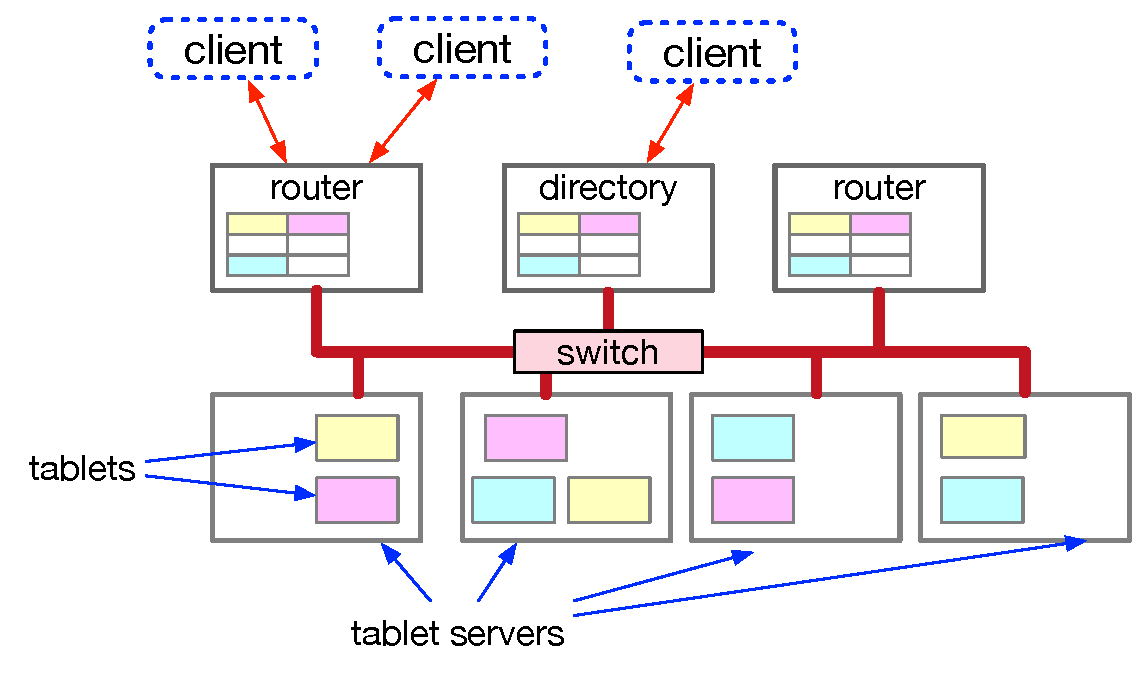
\includegraphics[width=0.75\textwidth]{figures/table_store_architecture.eps}
\end{center}

Small deployments will typically have a small number of physical nodes, each running multiple processes.

\begin{itemize}[-,noitemsep,topsep=-10pt]
\item Routing process: redirect requests based on partition attribute.
\item Data storage process: read/write operations on tuples.
\item Load re-balancing process.
\item Query/transaction execution process!
\end{itemize}
\end{frame}

%
%--------------------------------------------------------------------------------------------------------------
%

\begin{frame}{Updating the data}

Inserting new tuples requires choosing a primary tablet to hold the tuple and updating the directory accordingly.

To delete a tuple or to modify a non-partition attribute of a tuple, we:

\begin{enumerate}[(1),noitemsep,topsep=-5pt]
 \item Find the tablet with the \textbf{primary} copy of the tuple.
 \item Perform the update/deletion.
 \item Synchronize \alert{all replicas} of that partition.
 \end{enumerate} 

\vskip1em

Updating the partition attribute(s) is often implemented as deleting the tuple followed by an insertion of the ``modified'' one.
\end{frame}


%
%--------------------------------------------------------------------------------------------------------------
%
\begin{frame}{Synchronization}

Recall that in these systems data loss is prevented by having each tuple stored in multiple places. 

Which means we need to replicate every insertion and every update in the primary tablet to its replicas.

\vskip1em

\begin{block}{How do we ensure the replicas are \blue{synchronized}?}
\begin{itemize}[-,noitemsep]
\item \alert{Two-phase Commit (2PC) protocol}\footnotemark ensures synchronous and atomic updates across replicas.
\item Persistent-messaging implements a more relaxed, \textbf{eventual}, consistency model.
\end{itemize}
\end{block}

% \vskip1em

\footnotetext{\url{https://en.wikipedia.org/wiki/Two-phase_commit_protocol}}

\end{frame}

%
%--------------------------------------------------------------------------------------------------------------
%

\begin{frame}{Why do we need synchronization again?}

Synchronization is necessary (in single-node or multi-node systems) to ensure that transactions are atomic and durable and to ensure that the transaction schedule is conflict-serializable.

\vskip1em

In other words, \alert{synchronization is needed if we want ACID transactions}.

\vskip1em

\begin{block}{Not all applications need synchronization though...}

As we will discuss (soon) some applications can tolerate data inconsistencies as long as they can be (eventually) detected and corrected.

\vskip1em

\alert{\textbf{Trade-off:}} give up consistency to gain in speed.
\end{block}

\end{frame}

